\chapter{Анализ исходных данных, требований к их обработке и интеграционной поверхности модуля ранжирования цифровых профилей соискателей}
\label{chapter:data}

В главе описываются сбор, профилирование, очистка и разметка исходных данных, анализируются требования к конвейеру предварительной обработки и модулю семантического анализа, рассматриваются программный интерфейс ранжирующего сервиса и фактическая интеграционная поверхность с ядром Reqcore.
\section{Выполнение сбора, профилирования, очистки и разметки исходных данных вакансии и резюме}

Сбор текстовой информации в системе автоматизированного подбора персонала концептуально подразделяется на работу с двумя классами сущностей. С одной стороны, обрабатываются данные о вакансиях (должностные обязанности, формальные требования, стек технологий, условия труда). С другой стороны, обрабатываются данные о резюме (развернутый опыт работы, ключевые навыки, наличие сертификатов, данные об образовании, стаж работы). Практика систематического извлечения таких аспектов для целей ранжирования соискателей прямо описана в системе PROSPECT: из резюме выделяются навыки, опыт по навыкам, образование и прошлый профессиональный опыт, после чего эти признаки используются как фасеты и как дополнительная структурированная информация для поиска. Это методически оправдано, поскольку структурированные признаки уменьшают неоднозначность свободного текста: рекрутер и алгоритм могут отдельно сопоставить требуемый навык, длительность опыта и образование, а не полагаться только на совпадение слов в полном тексте резюме. Авторы PROSPECT указывают, что добавление извлеченной структурированной информации улучшило качество ранжирования примерно на 30\%, то есть проверяли пользу именно этой дополнительной структуры для задачи отбора кандидатов \cite{src03}.

В качестве экспериментальной базы настоящего исследования использован синтетический корпус данных на основе данных одного из популярных сервисов по поиску работы, включающий массив резюме (\textasciitilde{}17,3 ГБ, содержащий профили кандидатов с полями профессиональной специализации, стажа и зарплатных ожиданий), массив описаний вакансий (\textasciitilde{}44,9 ГБ, включающий текстовые описания, требования, условия и метаданные), а также журнал событий откликов соискателей на вакансии (\textasciitilde{}293 МБ), служащий ключевым источником для формирования обучающих текст вакансии и текст резюме. Каждая такая пара получает метку решения сотрудника найма: label = 1, если историческое событие показывает принятие кандидата к рассмотрению или приглашение на собеседование по данной вакансии, и label = 0, если зафиксирован отказ. На этих парах дообучается модель раздельного кодирования: оптимизация направлена на то, чтобы сближать векторные представления вакансий и резюме, по которым соискатель был одобрен к дальнейшему рассмотрению, и разводить векторы пар, где было отказано в дальнейшем рассмотрении кандидатуры на конкретную вакансию. Помимо основных вышеописанных массивов информации корпус данных содержит дополнительные таблицы профессиональных навыков, опыта работы, образования и иных атрибутов кандидатов. Масштаб корпуса обусловил необходимость реализации потокового конвейера обработки (streaming batch processing) с поддержкой разбиения на фрагменты (chunking): только два основных текстовых массива занимают около 62,2 ГБ, что превышает типичный объем оперативного запоминающего устройства локального рабочего места или малого серверного контура на 16-32 ГБ, а потому полная загрузка данных в оперативную память была бы нестабильной и невоспроизводимой.

Профилирование корпуса цифровых данных вакансий и резюме должно протоколировать распределение длины текста, долю шумовой или неинформативной информации (маркетинговые блоки, универсальные фразы), плотность доменных терминов, процентную долю смысловых дубликатов, а также языковой состав текстов резюме и вакансий. К доменным терминам в данной работе относятся не любые часто встречающиеся слова, а профессионально значимые обозначения: названия ролей (системный аналитик, backend-разработчик, специалист по подбору персонала), уровни позиции (стажер, Junior, Middle, Senior, Lead), технологии и инструменты (Python, SQL, Docker, Kubernetes, 1C), названия профессиональных областей (информационная безопасность, машинное обучение, кадровое администрирование), сертификаты и образовательные квалификации. В контексте извлечения навыков из резюме существенной проблемой признаются границы профессиональной терминологии: навыки можно описывать через экспертную таксономию ESCO, через американскую модель профессионального содержания O*NET, через внутренний словарь компании или через автоматически извлеченные кластеры терминов из корпуса вакансий. Такое разнообразие подходов к классификации навыков, должностей и квалификаций обуславливает необходимость строгих внутренних регламентов и унификации метрик для разметки данных \cite{src18, src30, src31}.

Процедура разметки массива данных в рамках данной работы протекает на нескольких уровнях:

\begin{compactenum}
  \item Разметка кадрового решения по паре текст вакансии и текст резюме для последующего обучения ранжирующих моделей и контроля качества по нормализованной дисконтированной кумулятивной выгоде (Normalized Discounted Cumulative Gain, NDCG). На этом уровне вся пара получает одну численную метку: значение 1 показывает, что резюме было фактически продвинуто сотрудником по подбору персонала в рамках конкретной вакансии, а значение 0 показывает отказ или отсутствие продвижения на следующий этап.
  \item Детализированная разметка терминов на уровне выделения текстовых фрагментов с типизацией навыков: технические навыки (hard skills), надпрофессиональные навыки (soft skills) и знания предметной области (knowledge skills). Выделение текстовых фрагментов означает, что аннотатор отмечает не весь документ целиком, а конкретные фрагменты текста, например Python, ведение переговоров или бухгалтерский учет. Такая разметка необходима для интерпретируемой выдачи: система может не только показать итоговый балл, но и объяснить, какие навыки в резюме совпали с требованиями вакансии.
  \item Косвенная разметка цифровых представлений резюме и вакансии посредством накопления поведенческих сигналов от сотрудников подбора персонала, собранных из системы автоматизированного подбора персонала. В этой схеме метка не ставится вручную в отдельном интерфейсе разметки, а выводится из событий воронки подбора: отказов в дальнейшем рассмотрении соискателя, приглашений на собеседование, перевода на следующий этап и других действий, которые отражают решение специалиста в промышленной эксплуатации системы автоматизированного подбора персонала \cite{src41, src42}.
\end{compactenum}

В практической реализации данной работы разметка соответствия текст вакансии и текст резюме осуществлялась на основе журнала событий откликов корпуса синтетических данных на основе данных сайта агрегатора вакансий и резюме: значение label = 1 присваивалось случаям, где кандидат был принят к рассмотрению или приглашен на собеседование по конкретной вакансии, а значение label = 0 присваивалось в случае фактов официального отказа со стороны специалиста по подбору персонала на сайте-агрегаторе. Использование реальных решений сотрудников по подбору персонала исключает необходимость генерации искусственных примеров отказа, не основанных на реальных событиях. Размеченный корпус данных разделен в пропорции 80\% (обучение), 10\% (валидация), 10\% (тестирование). Это не математически единственно возможное соотношение, а распространенная эвристика для отложенной проверки: большая часть данных передается модели для настройки параметров, отдельная меньшая часть используется для подбора порогов и контроля переобучения, а финальные 10\% остаются изолированным тестовым срезом, который не используется ни при обучении, ни при выборе порога.

Ключевым примером при решении задачи разметки наборов данных о резюме и вакансиях является ресурс SKILLSPAN: Hard and Soft Skill Extraction from English Job Postings, включающий 14,5 тыс. предложений из описаний вакансий и более 12,5 тыс. размеченных текстовых фрагментов навыков и знаний. Авторы вводят базовую модель BERT и сравнивают ее с моделями, дополнительно настроенными на языке вакансий, а также с вариантами для длинных фрагментов и многозадачного обучения; результат показывает, что доменно адаптированные модели лучше моделей без такой адаптации, а отдельная постановка задачи извлечения навыков лучше многозадачного варианта \cite{src24}. Аналогичная логика подтверждается работой conSultantBERT: Fine-tuned Siamese Sentence-BERT for Matching Jobs and Job Seekers, где сиамская модель Sentence-BERT дообучается на более чем 270 тыс. текст резюме и текст вакансии, размеченных консультантами по подбору персонала, и превосходит варианты на основе взвешенных признаков TF-IDF и базовых BERT-представлений \cite{src39}. Основываясь на этом, необходимо: а) актуализировать собственную таксономию навыков; б) выполнять настройку моделей с механизмом самовнимания на локальных корпусах данных, взятых из системы автоматизированного подбора персонала; в) оформлять модуль извлечения навыков из данных о резюме и вакансиях как независимый подпроцесс. Изоляция нужна потому, что ошибки извлечения навыков напрямую искажают последующее ранжирование: если навык не выделен или отнесен к неверной категории, модель ранжирования получает неполное представление профиля, а проверка качества итогового списка уже не позволяет понять, где возникла ошибка на этапе извлечения признаков или на этапе сортировки кандидатов \cite{src18, src24}.

По аналогии с работой CareerBERT: Matching Resumes to ESCO Jobs in a Shared Embedding Space for Generic Job Recommendations \cite{src01}, при наличии внутреннего резерва данных, то есть накопленной в системе автоматизированного подбора персонала истории резюме, вакансий, откликов и решений специалистов по найму, целесообразно использовать подходы лемматизации и стандартизации профессий по государственным классификаторам Российской Федерации, например Общероссийскому классификатору занятий ОК 010-2014 (МСКЗ-08) и Общероссийскому классификатору профессий рабочих, должностей служащих и тарифных разрядов, а также по международным таксономиям: европейской классификации навыков, компетенций, квалификаций и профессий ESCO и американской модели профессионального содержания O*NET \cite{src30, src31}. Механизм снижения терминологического разрыва состоит в нормализации разных формулировок к общему идентификатору профессии или набора навыков: например, разработчик на Python, backend engineer и программист серверной логики могут быть связаны с одной профессиональной категорией и пересекающимся набором навыков. После такой нормализации модель сравнивает не только исходные слова, но и стандартизированные признаки, поэтому резюме и вакансия остаются сопоставимыми даже при разных формулировках одного и того же опыта.

Ввиду наличия конфиденциальных персональных данных в резюме, а следовательно и в контуре программного комплекса, процедуры очистки данных должны включать деидентификацию. Исследования предвзятости в резюме и профессиональных биографиях показывают, что языковые модели и классификаторы способны использовать не только профессиональную информацию, но и косвенные социальные сигналы, включая пол, расу, университет, локацию или объем текста профиля; такие признаки могут влиять на выдачу даже тогда, когда они не должны быть основанием кадрового решения \cite{src22, src34, src35}. Корректная подготовка данных обязана скрывать параметры, не отражающие напрямую профессиональные качества соискателя, поскольку они повышают риск обучения модели на нежелательных прокси-признаках \cite{src02, src22}. В реализованном конвейере обработки данных маскирование персональных данных выполнено методом жесткой подстановки токенов: все обнаруженные паттерны телефонных номеров и адресов электронной почты заменяются соответственно на токены [MASKED\_PHONE] и [MASKED\_EMAIL], удаляются HTML-теги и шумовые спецсимволы, а пропущенные текстовые поля резюме и вакансий заполняются пустыми строками, чтобы последующие этапы сборки model\_input не прерывались на значениях null. Весь конвейер подготовки данных реализован по принципу пакетной обработки без внешних зависимостей на стандартной библиотеке Python, включая модули csv, sqlite3, re, json, pathlib и потоковое чтение файлов. Такой выбор снижает риск несовместимости окружения и позволяет обрабатывать корпуса объемом в десятки гигабайт на локальной конфигурации с 16-32 ГБ оперативной памяти или на малом сервере без загрузки полного объема информации в оперативное запоминающее устройство.

\section{Анализ требований к конвейеру предварительной обработки данных (preprocessing pipeline) и модулю вычисления семантической близости плотных векторных представлений текста}

Под конвейером предварительной обработки данных здесь понимается программная цепочка подготовки данных перед обучением модели для ранжирования цифровых профилей и последующим их ранжированием. Она последовательно принимает исходные тексты резюме и вакансии, очищает и нормализует текст, извлекает структурные признаки, например желаемую должность, уровень позиции, стек навыков, стаж, образование, опыт работы и зарплатные ожидания, собирает единое текстовое представление цифрового профиля соискателя для модели и подготавливает данные к расчету плотных векторных представлений текста:

\begin{compactenum}
  \item Модуль приема (ingestion): получение цифровых профилей кандидатов и текстовых описаний вакансий из базы данных системы автоматизированного подбора персонала, проверка структурного формата и нормализация кодировок текста. В целевой системе автоматизированного подбора персонала под названием Reqcore извлечение сырого текста из загруженных резюме осуществляется на основе типа файла MIME с привлечением специализированных библиотек парсинга (PDF, DOCX, DOC) языка программирования Python, после чего применяется эвристическая сегментация на смысловые секции (опыт работы, образование, навыки) посредством регулярных выражений по характерным паттернам заголовков, например регулярного выражения вида (см.~\ref{fig:regex-section}).
  \item Модуль лингвистической нормализации: токенизация строк, то есть разбиение текста на отдельные слова, числа, технологические обозначения и служебные разделители, удаление пунктуации и приведение текста к нижнему регистру (lowercasing) с сохранением значимых символов для найма сотрудников из сферы информационных технологий, например \path|+|, \# для обозначений C++, C\#. Модуль выявляет язык источника, производит дедупликацию повторяющихся блоков, например одинакового описания компании, скопированного во множество вакансий, удаляет юридические штампы и шаблонные кадровые блоки, например типовые фрагменты Обязанности:, Условия:, Описание вакансии:, при помощи регулярных выражений для снижения шума в последующих плотных векторных представлениях.
  \item Структурно-аналитический модуль: отвечает за вычленение смысловых кластеров, например, опыт работы, образование, навыки, и извлечение специализированных терминов по однородным категориям: технические навыки, надпрофессиональные навыки (soft skills) и образование. Такой программный модуль выполняет извлечение маркеров уровня квалификации соискателя (\path|Intern/Junior|, Middle, Senior, Lead) и ключевых технологических навыков (Python, SQL, Docker, Kubernetes и др.) с формированием структурированных JSON-списков. Формируется детальная цифровая матрица компетенций цифрового профиля соискателя \cite{src24}.
  \item Далее идет компонент конвертации нормализованных текстов в плотные векторные представления на базе модели векторных представлений предложений (Sentence Embeddings using Siamese Bidirectional Encoder Representations from Transformers Networks). Перед подачей в модель-кодировщик, то есть нейросетевой компонент, который преобразует текст в числовой вектор смысла, извлеченные признаки агрегируются в унифицированный текстовый формат вида Role: [роль] | Seniority: [уровень] | Skills: [список навыков] | Text: [очищенное описание]. Такой формат снижает неопределенность входа: модель получает не произвольный фрагмент текста, а явно размеченные зоны с ролью, уровнем позиции, навыками и общим описанием. Это помогает механизму самовнимания (Self-Attention), потому что одинаковые типы информации оказываются в повторяемых позиционных и смысловых контекстах: список навыков сравнивается со списком навыков, уровень позиции с уровнем позиции, а общий текст не смешивается с техническими маркерами. Доменная тонкая настройка внутри организации необходима тогда, когда локальные формулировки должностей, стек технологий и кадровые решения отличаются от общих корпусов предобучения; в этом случае модель учится сближать пары с подтвержденным продвижением кандидата и отделять их от с отказом \cite{src01, src06, src24}.
  \item Далее следует блок первичного поиска и формирования выборки, который реализует отбор узкой первичной выборки лучших кандидатов по критериям семантической схожести векторов. В планах развития данной работы осуществление подсчета схожести векторов через механизмы приближенного поиска ближайших соседей (Approximate Nearest Neighbor, ANN). Для этого в дальнейшей инфраструктуре потребуется система класса векторной базы данных (Vector Database), например векторная база данных Milvus, предназначенная для хранения плотных векторных представлений и поиска ближайших векторных объектов с фильтрацией \cite{src12}.
  \item Далее в планах развития идет модуль алгоритмического повторного ранжирования (Re-ranking): отвечает за финальный пересчет позиций первых N кандидатов при помощи алгоритмов обучения ранжированию (Learning to Rank). Учитываются и интегрируются исходные семантические оценки, например косинусное сходство вакансии и резюме в доменном векторном пространстве, выявленные структурные пересечения по профессиональному стажу, например совпадение требуемых 3+ года Python с периодами работы в резюме, и косвенные поведенческие метрики, например частота приглашений на интервью по похожим вакансиям, клики рекрутеров или перевод кандидата на следующий этап \cite{src17, src38, src43, src44, src45}.
  \item Далее модуль объяснимости (Explainability Engine) формирует интерпретируемые сводки (например, текстовые плашки совпадения навыков). Механизм прозрачности работы модели призван компенсировать фактор эффекта черного ящика, повышая доверие конечного пользователя (например, сотрудника по подбору персонала) внутри системы автоматизированного подбора персонала к результату алгоритма \cite{src23}.
  \item И наконец в дальнейшем завершающим шагом должен идти модуль генерации критериев оценки с использованием большой языковой модели: в целевой системе автоматизированного подбора персонала под названием Reqcore реализован автоматизированный конвейер формирования объективной шкалы оценивания кандидатов на основе текста описания вакансии. Система передает описание позиции в большую языковую модель с поддержкой нескольких провайдеров, включая OpenAI, Anthropic и Google Artificial Intelligence, и получает структурированный ответ, жестко валидируемый схемой JSON. Каждый сгенерированный критерий содержит уникальный идентификатор, наименование, инструкцию по поиску фактов в резюме, категорию критерия (технический навык, надпрофессиональный навык (soft skill) или образование), базовую шкалу оценки и рекомендованный вес значимости. Вес значимости показывает вклад критерия в итоговый балл: например, для вакансии разработчика Python критерий владения Python может получить вес 0,40, опыт работы с базами данных имеет вес 0,25, а коммуникационные навыки имеют вес 0,10. Полученные критерии далее выступают в роли формализованного чек-листа для автоматизированного оценивания входящих резюме под требования конкретной вакансии с использованием искусственного интеллекта.
\end{compactenum}

\begin{figure}[H]
\centering
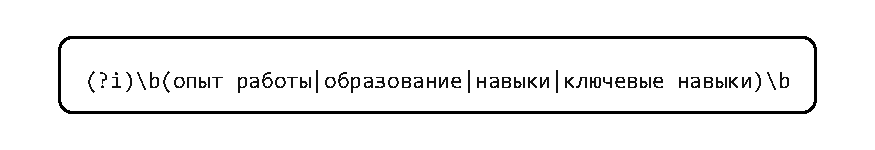
\includegraphics[width=0.92\textwidth]{figures/regex-section-headers.pdf}
\caption{Регулярное выражение для сегментации заголовков секций резюме}
\label{fig:regex-section}
\end{figure}

\section{Анализ программного интерфейса приложения (Application Programming Interface) и программных модулей интеграции модуля ранжирования соискателей с ядром системы автоматизированного подбора персонала}

Модуль программного интерфейса приложения (Application Programming Interface, API), работающий поверх протокола передачи гипертекста (Hypertext Transfer Protocol, HTTP), реализован в файле \path|experiments/scripts/11_api_server.py| как микросервис на фреймворке языка Python под названием FastAPI; в коде сервиса он имеет техническое имя ATS Semantic Ranking Engine API версии с названием 1.0.0. Выбор схем входных данных через классы CandidatePayload и SearchPayload связан не только с внутренним устройством кода: в документации FastAPI входное тело запроса описывается через модели Pydantic, а документация Pydantic прямо связывает такие модели с проверкой данных на основе аннотаций типов языка Python \cite{src48, src49}. В текущей реализации CandidatePayload это модель входного тела запроса для загрузки одного профиля кандидата: она требует строковый идентификатор id, подготовленный текст профиля model\_input и допускает необязательный словарь метаданных metadata для фильтрации. SearchPayload это модель входного тела запроса на ранжирование для маршрута \path|/search/rank|: она содержит текст вакансии vacancy\_text, необязательные фильтры по метаданным filters и параметр top\_k, задающий, сколько кандидатов с наибольшей оценкой семантического соответствия вернуть после сортировки по убыванию match\_score. Под маршрутом здесь понимается конкретная пара метода протокола передачи гипертекста и адреса программного интерфейса, например POST \path|/search/rank|, к которой внешний сервис может отправить запрос. Кроме схем Pydantic, при старте сервиса создаются две рабочие сущности. Первая это CANDIDATE\_INDEX: временный список словарей с кандидатами, добавленными через маршрут \path|/index/candidate|; он существует только в памяти запущенного процесса в Python и служит набором кандидатов, по которому затем выполняется ранжирование. Второй является объект ранжирования ATSRanker, загружаемый при старте приложения и выполняющий расчет косинусного сходства. Кандидатский профиль передается в программный интерфейс в уже подготовленном текстовом формате model\_input: это единая строка с ролью, уровнем, навыками и очищенным текстом резюме, которую модель использует как вход для построения векторного представления цифрового профиля кандидата. Отдельные публичные маршруты, которые по отдельному запросу возвращали бы только векторное представление вакансии или только векторное представление резюме без ранжирования, в коде не реализованы.

\begingroup
\setlength{\tabcolsep}{3pt}
\renewcommand{\arraystretch}{1}
{\linespread{1}\selectfont
\begin{longtable}{|P{0.17\textwidth}|P{0.06\textwidth}|P{0.20\textwidth}|P{0.27\textwidth}|P{0.20\textwidth}|}
\caption{Спецификация API-маршрутов FastAPI-сервиса ранжирования}\label{tbl:api}\\
\hline
Маршрут & Метод & Входная схема & Реализованное поведение & Ответ \\
\hline
\endfirsthead
\hline
Маршрут & Метод & Входная схема & Реализованное поведение & Ответ \\
\hline
\endhead
\hline
\endfoot
\hline
\endlastfoot
\path|/index/candidate| & POST & CandidatePayload: id, model\_input, metadata & Формирует словарь кандидата, добавляет обязательные поля id и model\_input, при наличии объединяет их с metadata, затем помещает запись во временный индекс CANDIDATE\_INDEX. & JSON со статусом indexed и числом записей total\_pool\_size. \\
\hline
\path|/search/rank| & POST & SearchPayload: vacancy\_text, filters, top\_k & Проверяет наличие загруженного RANKER\_ENGINE и вызывает метод search объекта ATSRanker для текущего CANDIDATE\_INDEX с учётом текста вакансии, фильтров и ограничения top\_k. & При незагруженной модели возвращает HTTP 500 с ошибкой Model not loaded; при штатном выполнении возвращает JSON, сформированный модулем ранжирования. \\
\hline
\path|/score| & POST & ScorePayload: vacancy\_text, candidate\_text & Преобразует одну текстовую пару текст вакансии и текст резюме через текущую модель RANKER\_ENGINE в два векторных представления, вычисляет косинусное сходство и возвращает одиночный match\_score. Используется как внутренний межсервисный маршрут для ветки provider === 'biencoder' в системе автоматизированного подбора персонала под названием Reqcore. & JSON со статусом ok, значением match\_score и временем latency\_ms либо HTTP 500 с ошибкой Model not loaded. \\
\end{longtable}
}
\endgroup

Таким образом, в текущем коде реализованы три маршрута, то есть три адреса программного интерфейса, доступные по протоколу передачи гипертекста: POST \path|/index/candidate| добавляет цифровой профиль кандидата во временный индекс, POST \path|/search/rank| ранжирует текущий набор кандидатов относительно данной вакансии, а POST \path|/score| используется как внутренний интеграционный маршрут для системы автоматизированного подбора персонала под названием Reqcore. Под временным индексом понимается список загруженных кандидатских профилей в оперативной памяти процесса Python: он существует только пока запущен сервис и не сохраняется в отдельную базу данных после перезапуска. Маршруты POST \path|/rank|, POST \path|/embed/job|, POST \path|/embed/resume|, POST \path|/index/upsert|, POST \path|/index/delete| и POST \path|/monitoring/log| в текущем коде отсутствуют.

В текущей версии программного интерфейса реализован базовый набор маршрутов, обеспечивающий индексацию кандидатских профилей, ранжирование текущего набора кандидатов относительно конкретной вакансии и вычисление одиночной оценки семантического соответствия для пары текст вакансии и текст резюме в сервисной интеграции с системой автоматизированного подбора персонала под названием Reqcore. Эта оценка показывает, насколько текст резюме близок требованиям конкретной вакансии в доменном векторном пространстве, сформированном моделью после тонкой настройки на кадровых событиях, а не в произвольном общеязыковом смысле. Она не является самостоятельным кадровым решением. Поэтому дальнейшее развитие программного интерфейса целесообразно связывать с практическими ограничениями прототипа: сейчас данные живут только в памяти процесса, а значит теряются при перезапуске сервиса; векторные представления не предрассчитываются отдельным маршрутом, поэтому один и тот же профиль приходится кодировать повторно; результаты работы модели не журналируются как эксплуатационные события, поэтому сложнее расследовать изменения выдачи после обновления модели или данных.

Одним из таких направлений может стать введение отдельных публичных маршрутов для работы с векторными представлениями текстов вакансий и резюме, то есть с числовыми векторными представлениями их смысла. В отличие от текущей реализации, где кандидатский профиль поступает в систему уже в подготовленном текстовом виде, выделение специализированных маршрутов для получения векторных представлений позволило бы формализовать этап предрасчета признаков, упростить инкрементальное обновление векторных представлений и сделать программный интерфейс более пригодным для сценариев, в которых этап подготовки данных отделен от этапа ранжирования. Для микросервисной архитектуры это важно потому, что подготовка плотных векторных представлений, хранение индекса, ранжирование и мониторинг могут обновляться, масштабироваться и откатываться независимо: например, модель можно переобучить и пересчитать векторы без изменения серверного ядра системы автоматизированного подбора персонала \cite{src32, src33}.

Перспективным направлением также является развитие механизмов синхронизации индекса. В текущем состоянии используется временный индекс в оперативной памяти (in memory), достаточный для демонстрации и проверки базовой логики поиска, однако в дальнейшем программный интерфейс может быть дополнен операциями обновления и удаления записей, ориентированными на согласованную синхронизацию между системой автоматизированного подбора персонала и внешним хранилищем векторных представлений цифровых профилей кандидатов. Реализация такого слоя позволила бы перейти от эпизодической загрузки данных к управляемому жизненному циклу профилей в системе и тем самым приблизить решение к требованиям промышленной эксплуатации: сохранению индекса после перезапуска сервиса, удалению устаревших резюме, обновлению профиля при изменении данных кандидата, контролю версий модели и воспроизводимому восстановлению состояния после сбоя \cite{src12, src32, src33}.

Отдельного развития требует и уровень прикладной наблюдаемости. В настоящей версии программного интерфейса отсутствует специализированный маршрут для журналирования результатов работы модели, а потому сбор сведений о качестве выдачи, динамике ранжирования и устойчивости поведения системы остается ограниченным. В дальнейшем целесообразно предусмотреть средства централизованной регистрации агрегированных метрик и служебных событий ранжирования, что создаст основу для систематического мониторинга, сравнительного тестирования версий модели и более прозрачной интерпретации результатов в эксплуатационной среде. Это позволит быстрее обнаруживать деградацию качества после обновления модели или корпуса данных, сопоставлять версии алгоритма между собой и аргументированно объяснять изменения выдачи специалистам по подбору персонала.

Наконец, дальнейшее расширение возможно на уровне маршрута ранжирования POST \path|/search/rank|, то есть адреса программного интерфейса, который принимает текст вакансии, текущий набор кандидатов и возвращает отсортированный список. Сейчас выдача содержит статус выполнения, задержку, сведения о примененных фильтрах, число рассмотренных кандидатов и массив результатов с идентификатором кандидата, числовой оценкой match\_score, то есть оценкой семантического соответствия резюме требованиям вакансии в доменном векторном пространстве, и короткой текстовой сводкой. В перспективе программный интерфейс может быть дополнен более богатым выходным форматом: версией модели, временем построения плотных векторных представлений, списком совпавших навыков, объяснением основных факторов ранжирования, информацией о примененных жестких фильтрах и ссылкой на сохраненный аудит расчета. Под аудитом расчета понимается отдельная запись с идентификатором запроса, временем запуска, версией модели, примененными фильтрами, числом рассмотренных кандидатов и итоговыми оценками, по которой можно восстановить, почему конкретный кандидат получил конкретную позицию в выдаче. Подобное развитие позволило бы сделать систему удобнее для практического использования в сценариях автоматизированного подбора персонала, где важна не только численная оценка соответствия кандидата, но и возможность объяснить основания, по которым профиль оказался выше или ниже в итоговом ранжированном списке цифровых профилей кандидатов.

\section{Анализ интеграционной поверхности системы автоматизированного подбора персонала под названием "Reqcore" с модулем семантического ранжирования цифровых профилей соискателей}

Текущая серверная точка интеграции между системой автоматизированного подбора персонала под названием Reqcore и модулем семантического ранжирования цифровых профилей соискателей реализована в обработчике \path|ats/reqcore/server/api/applications/[id]/analyze.post.ts|. Под обработчиком здесь понимается серверная функция маршрута, которая выполняется при запросе анализа конкретной заявки кандидата на вакансию и связывает данные из базы Reqcore с выбранным способом автоматизированной оценки. Reqcore в данной работе рассматривается как тестовый контур системы автоматизированного подбора персонала не потому, что сама система не является автоматизированной системой подбора персонала, а потому, что проверка выполнялась в локальном демонстрационном окружении, а не в промышленной эксплуатации у реальных пользователей. В этом контуре хранятся вакансии, резюме, отклики кандидатов на вакансии, критерии оценки цифровых профилей от сотрудников по подбору персонала, результаты анализа резюме соискателей и конфигурация провайдера искусственного интеллекта на уровне организации. Обработчик запускается при анализе одного отклика от соискателя на вакансию: он загружает данные резюме соискателя и активную конфигурацию из таблицы ai\_config, где хранится выбранный провайдер, название модели и параметры стоимости. Поле provider этой конфигурации определяет, каким способом считать итоговый балл соответствия резюме требованиям вакансии. Если выбран провайдер большой языковой модели, система идет по критериальному пути с объяснениями; если выбран вариант biencoder, система обращается к локальному сервису раздельного кодирования. В обоих вариантах результат интеграции сводится к обновлению поля \path|application.score|, то есть агрегированного числового балла заявки в таблице откликов, и к записи analysis\_run, то есть аудиторской записи о запуске анализа, выбранном провайдере, модели и служебных параметрах расчета. Различается только способ получения этого числа и объем сохраняемого объяснения.

Основной путь системы автоматизированного подбора персонала под названием Reqcore в текущей реализации ориентирован на большую языковую модель. Обработчик \path|analyze.post.ts| загружает заявку кандидата, конфигурацию искусственного интеллекта организации, критерии оценки из таблицы scoring\_criterion и текст резюме из поля \path|document.parsedContent|, затем вызывает функцию scoreApplication() из \path|ats/reqcore/server/utils/ai/scoring.ts|. Эта функция формирует структурированный запрос к модели по вакансии, критериям и информации о кандидате и передает его в generateStructuredOutput() из \path|ats/reqcore/server/utils/ai/provider.ts|, где выбирается конкретный внешний или совместимый провайдер большой языковой модели, например openai, anthropic, google или openai\_compatible. Возвращенный структурированный ответ содержит массив evaluations: поле criterionKey связывает оценку с конкретным критерием, applicantScore хранит балл кандидата по этому критерию, confidence отражает уверенность модели, evidence содержит подтверждающие фрагменты резюме, strengths перечисляет сильные стороны, а gaps фиксирует недостающие признаки. После этого тот же обработчик \path|analyze.post.ts| вычисляет итоговый балл через computeCompositeScore(), сохраняет детальные оценки по критериям в таблицу criterion\_score, а агрегированный результат записывает в поле \path|application.score|.

Альтернативный путь интеграции реализован как ветка при выполнении условия provider === 'biencoder' в том же файле \path|analyze.post.ts|. В этой ветке система автоматизированного подбора персонала под названием Reqcore не вызывает провайдер большой языковой модели и не использует scoreApplication(), то есть не запускает критериальную оценку большой языковой моделью с объяснениями. Вместо этого обработчик вызывает локальную вспомогательную функцию scoreWithBiEncoder(), объявленную в этом же серверном обработчике для связи с внешним сервисом ранжирования, написанным на языке Python. Функция получает адрес сервиса из переменной окружения операционной системы BIENCODER\_URL: эта переменная задается при запуске Reqcore и указывает базовый адрес сервиса ATS Semantic Ranking Engine API, реализованного в файле \path|experiments/scripts/11_api_server.py|, куда нужно отправлять запросы по протоколу передачи гипертекста (HTTP). Затем функция отправляет POST-запрос по протоколу HTTP на маршрут \path|/score| с телом запроса \{ vacancy\_text, candidate\_text \}. Модуль семантического ранжирования вакансий и резюме загружает ATSRanker, то есть класс-обертку над моделью Sentence Transformer и логикой фильтрации/сортировки кандидатов, преобразует текст вакансии и текст резюме в два отдельных плотных векторных представления и вычисляет косинусное сходство между ними. В ответ возвращается match\_score, которая являеться числовой оценкой семантического соответствия резюме требованиям вакансии в доменном векторном пространстве. Затем \path|analyze.post.ts| линейно отображает эту числовую оценку из диапазона [-1, 1] в шкалу 0..100 и записывает результат в \path|application.score|, то есть итоговый балл заявки. Для этой ветки массив evaluations остается пустым, а записи в criterion\_score не создаются, поскольку путь раздельного кодирования вакансии и резюме (bi-encoder) предназначен для предварительного числового отбора кандидатов или альтернативной грубой оценки соответствия, а не для замены полного критериального анализа с использованием большой языковой модели.

Следовательно, фактическая точка интеграции находится не в пользовательском интерфейсе (User Interface) и не в клиентском коде, а в серверном маршруте анализа заявки \path|ats/reqcore/server/api/applications/[id]/analyze.post.ts|. С точки зрения структуры взаимодействия это означает, что обе стратегии оценки используют одну и ту же бизнес-сущность заявки и одно и то же поле итогового балла \path|application.score|, но различаются глубиной интерпретации: путь с большой языковой моделью сохраняет детальные объяснения по критериям в criterion\_score, а путь biencoder возвращает только одну числовую оценку семантического соответствия пары текст вакансии и текст резюме. Поэтому путь biencoder корректно описывать как альтернативный или предварительный путь ранжирования, пригодный для дешевого первичного отбора откликнувшихся кандидатов, но не как полную замену всей логики большой языковой модели в системе Reqcore.

Компактная схема развертывания текущей интеграции имеет вид:

\FloatBarrier
\begin{figure}[H]
\centering
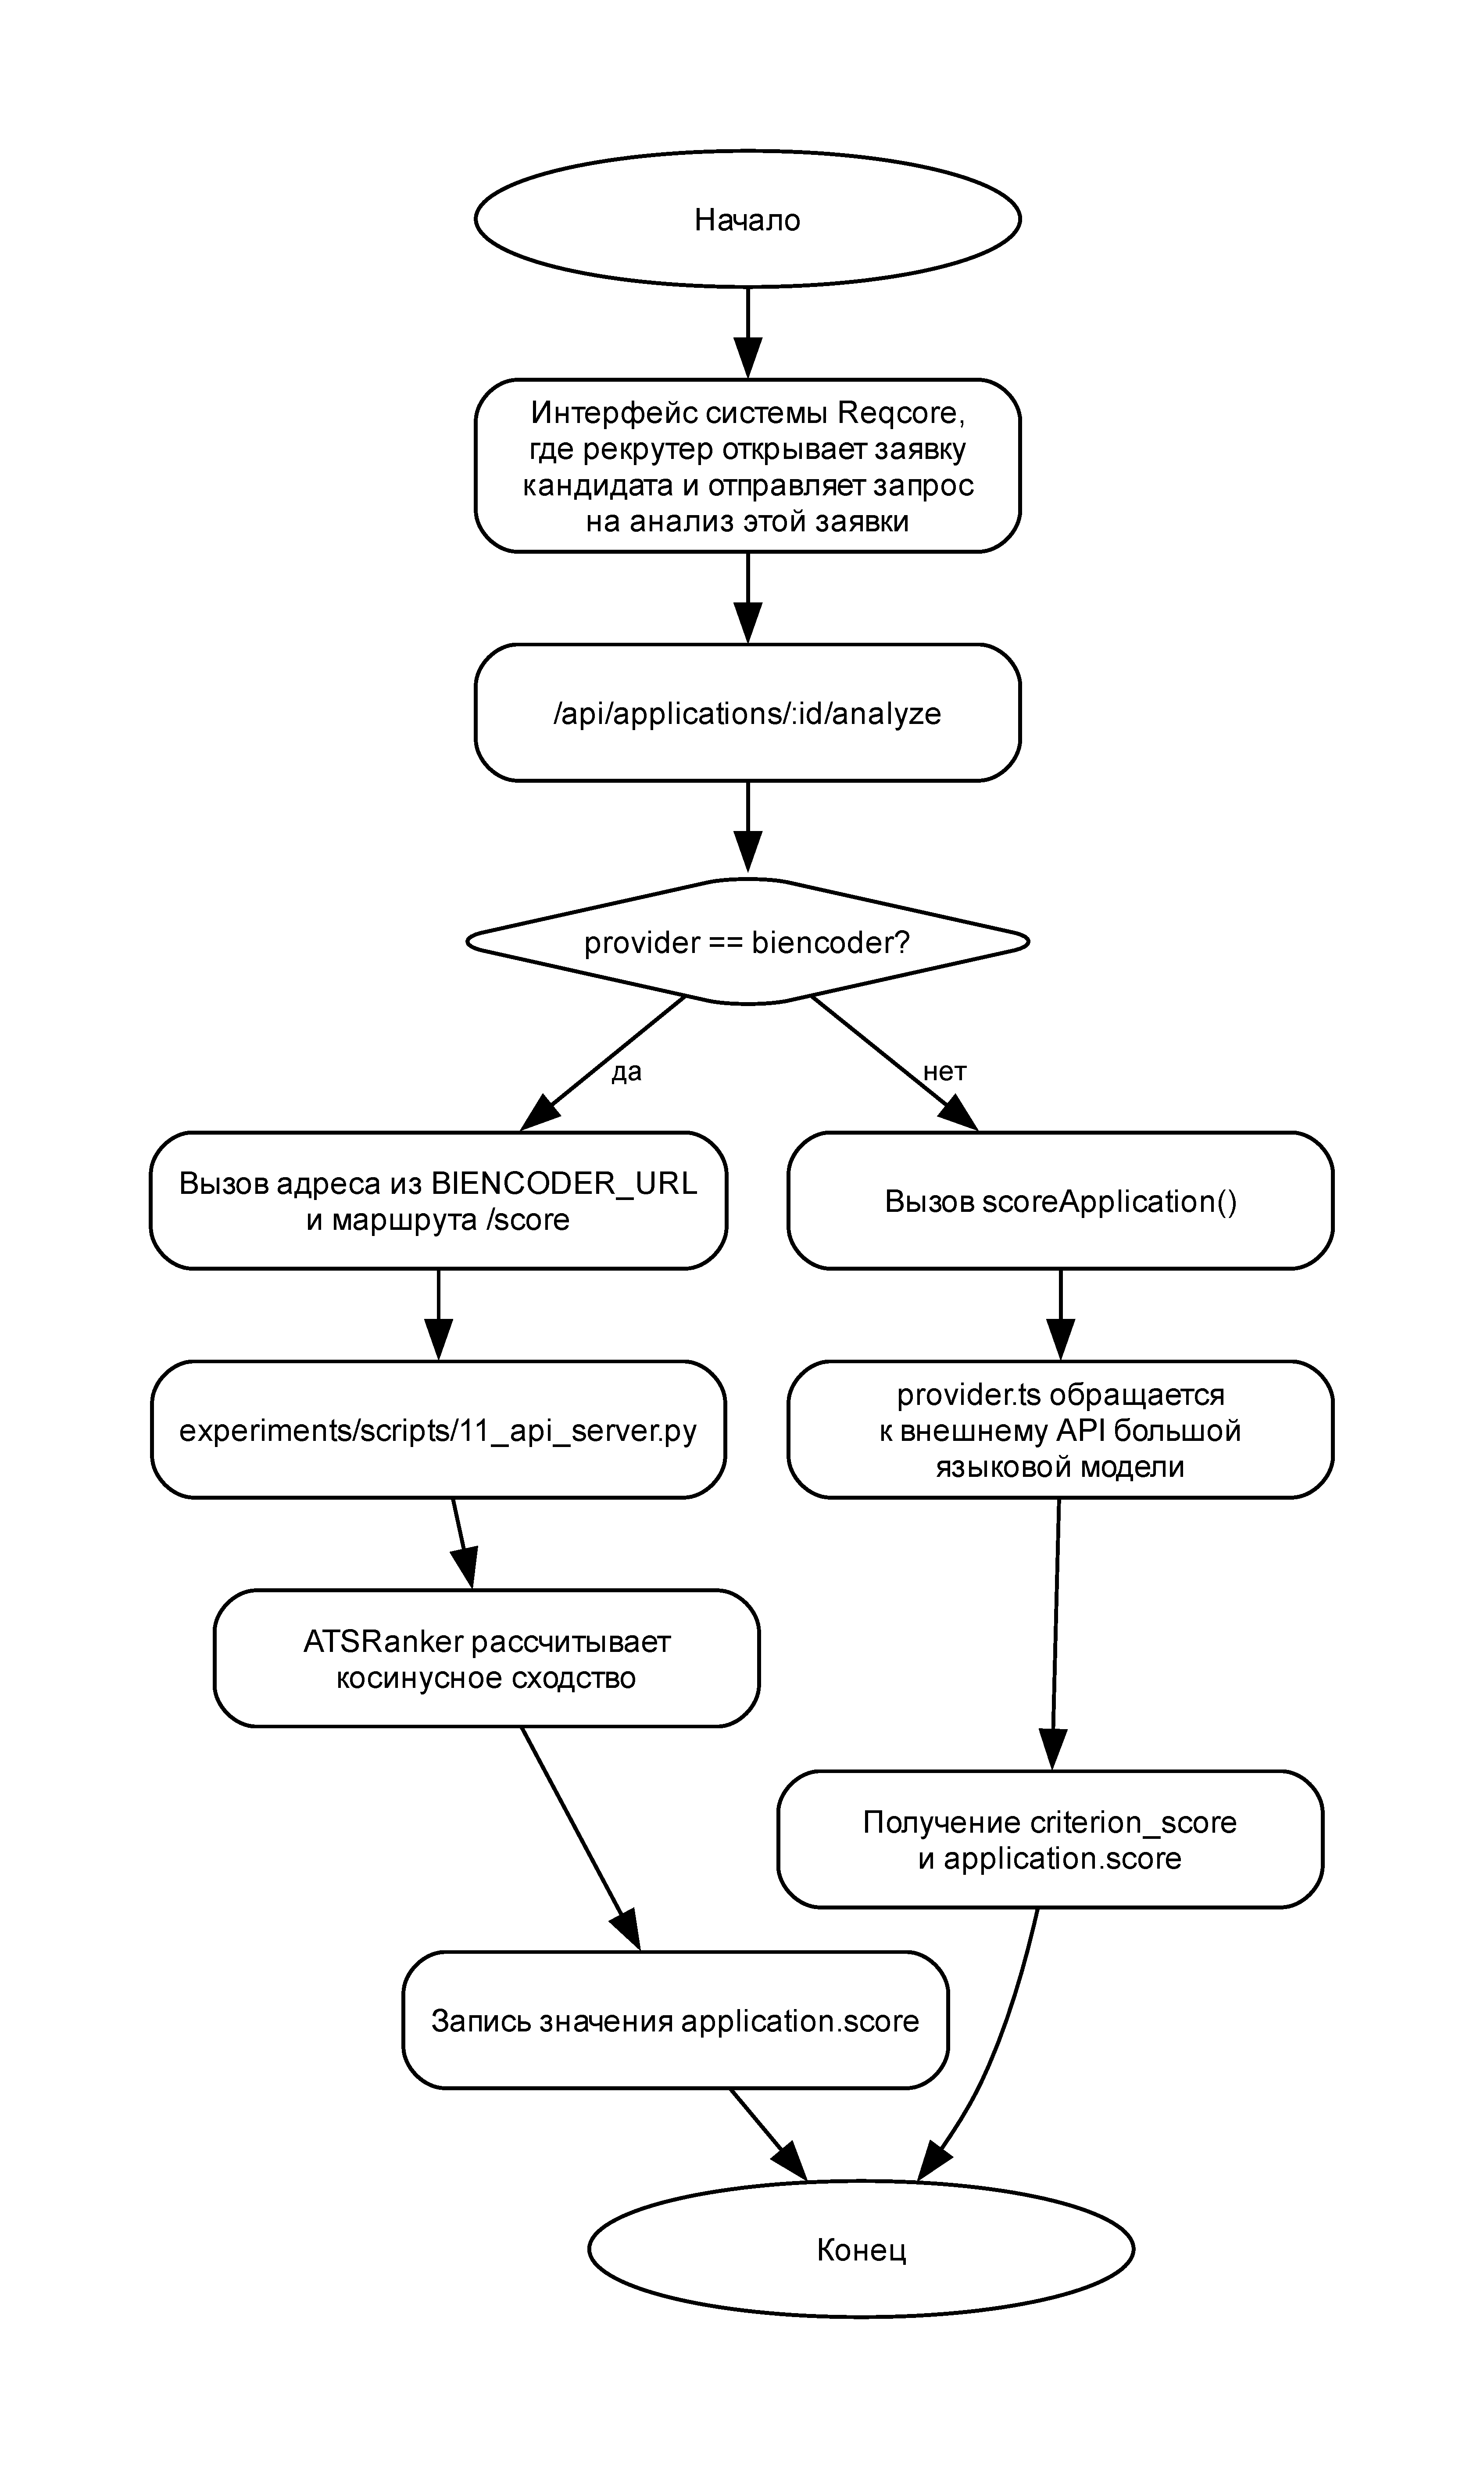
\includegraphics[width=\textwidth,height=0.648\textheight,keepaspectratio]{figures/application_analysis_request_flow.pdf}
\caption{Поток обработки запроса анализа заявки в интеграции Reqcore с модулем ранжирования}
\label{fig:flow}
\end{figure}

В реализованном программном контуре затронуты следующие файлы: \path|ats/reqcore/server/api/applications/[id]/analyze.post.ts| как основная точка маршрутизации, \path|ats/reqcore/server/utils/ai/scoring.ts| как механизм оценивания с использованием большой языковой модели, \path|ats/reqcore/server/utils/ai/provider.ts| как адаптер провайдера, \path|ats/reqcore/server/database/schema/app.ts| как место определения таблиц criterion\_score, analysis\_run и поля \path|application.score|; \path|experiments/scripts/11_api_server.py| как модуль расчета семантической близости резюме требованиям вакансии через модель раздельного кодирования (bi-encoder). Именно эти файлы образуют фактическую интеграционную поверхность между системой автоматизированного подбора персонала под названием Reqcore и модулем семантического ранжирования: модуль принимает подготовленные тексты вакансии и резюме, вычисляет доменную оценку соответствия, возвращает ее через HTTP-интерфейс и позволяет Reqcore сохранить результат в существующем контуре анализа заявки.

\section{Выводы}

\begin{compactenum}
  \item Для решения поставленной задачи во второй главе обоснована структура конвейера, который разделяет сбор и очистку данных, извлечение признаков, формирование входа модели, вычисление векторных представлений и ранжирование кандидатов.
  \item Подготовка данных должна включать деидентификацию и нормализацию текстов, поскольку персональные и шумовые признаки могут искажать обучение модели и повышать риск нежелательных прокси-зависимостей.
  \item Анализ FastAPI-сервиса фиксирует минимальный интерфейс прототипа: индексацию кандидатских профилей, ранжирование набора кандидатов и расчет одиночной оценки соответствия пары вакансия резюме.
  \item Интеграционная поверхность Reqcore описана как альтернативный серверный путь расчета числового балла, который не заменяет критериальную оценку большой языковой моделью, а дополняет ее более дешевым предварительным ранжированием.
\end{compactenum}
